% ============================================================================
\section{Neural end-to-end TTS}
% ============================================================================

\begin{frame}{2016--2021 Era: The Neural Revolution (WaveNet)}
    \begin{itemize}
        \item Deep generative model for raw audio
        \item Autoregressive: predicts next sample given previous samples
        \item High-quality, natural-sounding speech
        \item Equation:
        \[
            p(x) = \prod_{t=1}^{T} p(x_t | x_{1}, ..., x_{t-1})
        \]
        \item Computationally expensive for real-time use
    \end{itemize}
\end{frame}

\begin{frame}{2016--2021 Era: The Neural Revolution (WaveNet)}
    \centering
    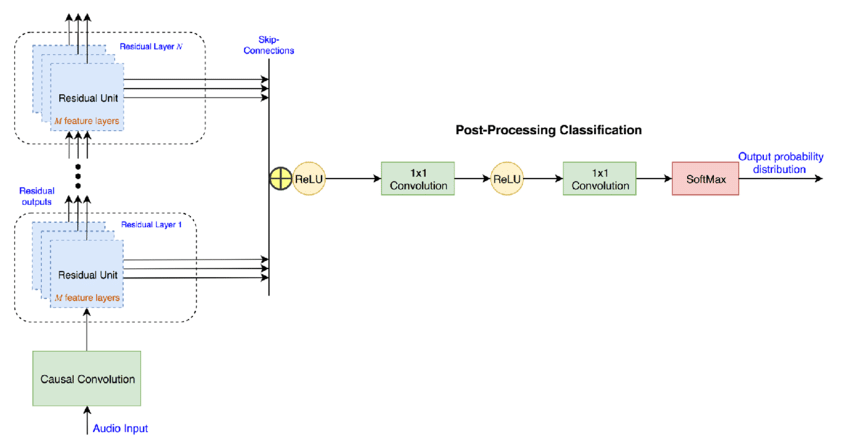
\includegraphics[width=\textwidth,height=0.72\textheight,keepaspectratio]{images/audio-nlp/wavenet_architecture.png}
    \slideimgsource{WaveNet architecture, redrawn by a third party (the paper's own Fig.~4 is a different, more compact drawing); architecture from van den Oord et al., ``WaveNet: A Generative Model for Raw Audio,'' \href{https://arxiv.org/abs/1609.03499}{arXiv:1609.03499}.}
\end{frame}

\begin{frame}{2016--2021 Era: Neural vocoders (WaveNet and beyond)}
  \begin{itemize}\footnotesize
    \item Mel-spectrograms show how frequencies change over time, but must be turned back into sound waveforms.
    \item Griffin-Lim was the early answer: recover the missing phase from a magnitude spectrogram by iterating between the time and frequency domains. Cheap, but the quality was limited.
    \item Neural vocoders like WaveNet can reach human-level speech quality.
    \item WaveNet generates raw audio samples one at a time: 16,000 per second in the original paper, 24,000 in the Tacotron~2 vocoder.
    \item It uses dilated causal convolutions, so it can ``see'' a lot of context efficiently.
    \item WaveNet models the conditional probability of each sample: \[
      p(\mathbf{x} \mid \mathbf{h}) = \prod_{t=1}^{T} p(x_t \mid x_1, \dots, x_{t-1}, \mathbf{h})
    \]
    where $\mathbf{h}$ is the mel-spectrogram.
    \item This approach gives very natural speech, but it is slow to run for real-time use.
  \end{itemize}
\end{frame}

\begin{frame}{2016--2021 Era: End-to-end Neural TTS (Tacotron)}
  \centering
  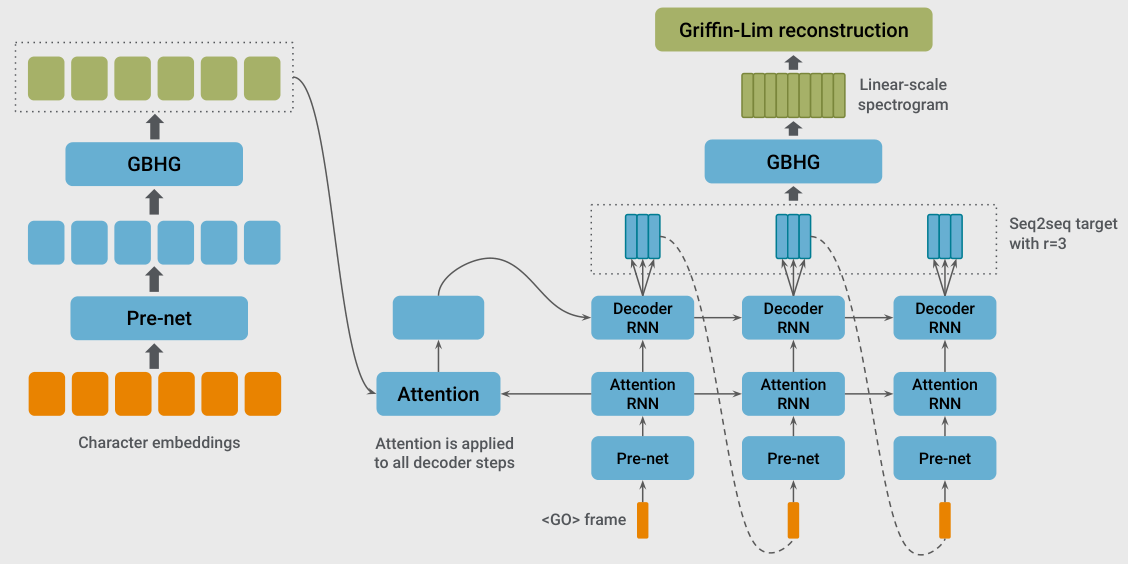
\includegraphics[width=0.95\textwidth,height=0.66\textheight,keepaspectratio]{images/tts/tts_tacotron_architecture.png}
  \slideimgsource{Stanford CS224S, Lecture 1 (2024 Spring), slide 31, redrawing Wang et al., ``Tacotron: Towards End-to-End Speech Synthesis,'' \href{https://arxiv.org/abs/1703.10135}{arXiv:1703.10135}, Fig.~1. Characters in, raw spectrogram out, then Griffin-Lim to synthesize speech. The ``GBHG'' boxes are the slide's typo for CBHG (1-D convolution bank, highway network, bidirectional GRU).}
\end{frame}

\begin{frame}{Tacotron 2}
    \begin{itemize}
        \item End-to-end TTS system
        \item Pipeline:
        \begin{itemize}
            \item Text $\rightarrow$ Mel-spectrogram (sequence-to-sequence model)
            \item Mel-spectrogram $\rightarrow$ WaveNet/GAN vocoder (audio synthesis)
        \end{itemize}
        \item Improved prosody and pronunciation
        \item Flexible for different voices and languages
    \end{itemize}
\end{frame}

\begin{frame}{Tacotron 2}
    \centering
    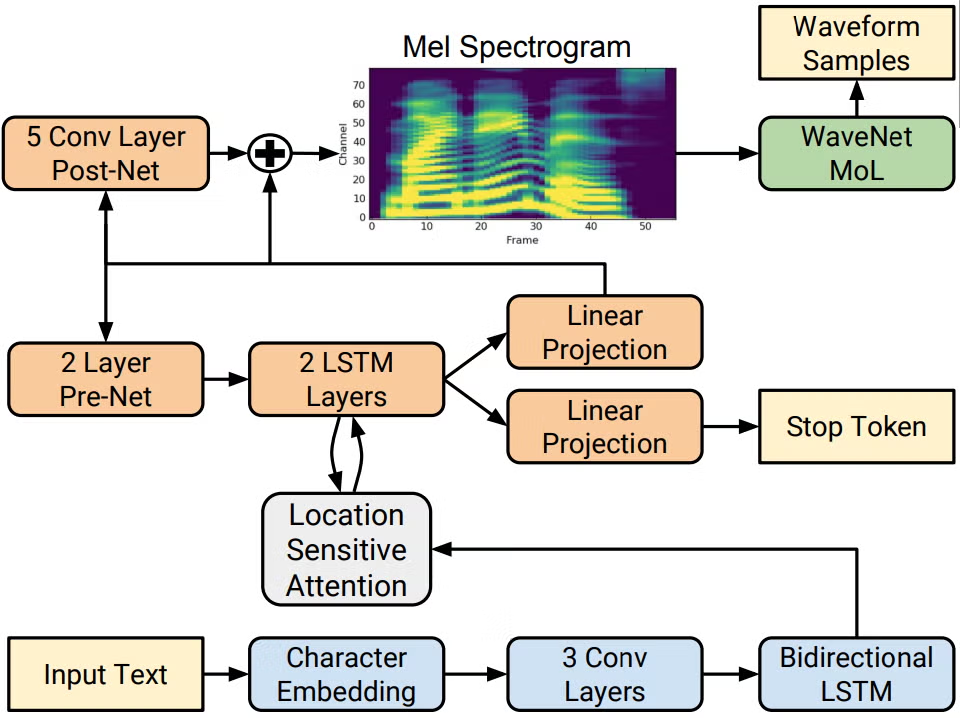
\includegraphics[width=\textwidth,height=0.72\textheight,keepaspectratio]{images/audio-nlp/tacotron2_pipeline.png}
    \slideimgsource{Shen et al., ``Natural TTS Synthesis by Conditioning WaveNet on Mel Spectrogram Predictions'' (Tacotron~2), Fig.~1; \href{https://arxiv.org/abs/1712.05884}{arXiv:1712.05884}.}
\end{frame}

\begin{frame}{Autoregression: the deployment bottleneck}
  \begin{itemize}\footnotesize
    \item \textbf{Latency:} Tacotron~2 with a WaveNet-class vocoder raised fidelity but blocked low-latency, on-device synthesis: one frame, then one sample, at a time.
    \item \textbf{Robustness:} the soft attention linking text to frames can also break down, so hard inputs come out with \textbf{skipped or repeated words}. Predicting an explicit duration per phoneme instead nearly removes those failures, and it is why later models search for a hard monotonic alignment rather than learning a soft one.
    \item Both problems point the same way: \textbf{non-autoregressive (NAR)} acoustic models and fast vocoders. FastSpeech reports mel generation $270\times$ faster and end-to-end synthesis $38\times$ faster than its autoregressive Transformer TTS teacher.
  \end{itemize}
\end{frame}
